\documentclass[11pt, oneside]{article}   	% use "amsart" instead of "article" for AMSLaTeX format
\usepackage[margin=1in]{geometry}                		% See geometry.pdf to learn the layout options. There are lots.
\geometry{letterpaper}                   		% ... or a4paper or a5paper or ... 
%\geometry{landscape}                		% Activate for rotated page geometry
%\usepackage[parfill]{parskip}    		% Activate to begin paragraphs with an empty line rather than an indent
\usepackage{graphicx}				% Use pdf, png, jpg, or eps§ with pdflatex; use eps in DVI mode
								% TeX will automatically convert eps --> pdf in pdflatex		
\usepackage{amssymb}
\usepackage{awesomebox}
%SetFonts

%SetFonts

\usepackage{amsmath}
\DeclareMathOperator{\plainmod}{\text{ mod }}
\let\emptyset\varnothing

\newcommand{\reals}{\mathbb{R}}
\newcommand{\realsText}{$\mathbb{R}$}
\newcommand{\ints}{\mathbb{Z}}
\newcommand{\intsText}{$\mathbb{Z}$}

\title{Homework 5}
\author{Discrete Structures 1}
\date{due: 13 April 2023, 8:00am}							% Activate to display a given date or no date

\begin{document}
\maketitle
%\section{}
%\subsection{}

Your task for this homework will be to answer the following questions without using any calculating resources. 
Your responses should be submitted via blackboard by the due date above as a PDF (submissions in any other format will be returned to the user and a resubmissions will be requested). 
You are free to use whatever tools you would like to generate the response document: 
scanned hand-written paper, 
tablet generated hand-written, 
microsoft word (with this option, please use the equation editor to correctly format your responses), 
\LaTeX, etc.
Your TA, IA, and Instructor are available to help during their designated office hours or via email 
(note that emails sent during non-business hours may not be responded to until the next working day). 

%\importantbox{
%\textbf{Note:} all of these questions are on topics from chapters 5; thus you will only be proving by induction in this homework assignment. 
%}
\begin{enumerate}
% 3.148-151
\item Let $F$ denote the set of all functions $f : \reals \rightarrow \reals$ taking real numbers as input and producing real numbers as output. 
(For one example, $plusOne(x) = x + 1$ is a function $plusOne : \reals \rightarrow \reals$, so $plusOne\in F$.) 
Determine the truth of the following propositions, and justify your answer. 
\begin{enumerate}
\item $\forall c \in \reals \left[\exists f \in F : f(0) = c\right]$
\item $\exists f \in F \left[\forall c \in \reals : f(0) = c\right]$
\item $\forall c \in \reals \left[\exists f \in F : f(c) = 0 \right]$
\item $\exists f \in F \left[\forall c \in \reals : f(c) = 0 \right]$
\end{enumerate}

%3.160-163
\item 
Let $P \in \left\{0,1\right\}^{n\times m}$ be a 2-dimensional array of the pixels of a black-and-white image: 
for every $x$ and $y$, the value of $P[x, y] = 0$
if the $\langle x, y\rangle$-th pixel is black, and $P[x, y] = 1$ if it’s white. 
Translate these statements into predicate logic:
\begin{enumerate}
\item Every pixel in the image is black
\item There is at least one white pixel
\item Every row has at least one white pixel
\item There are never two consecutive white pixels in the same column
\end{enumerate}

%3.168
\item According to Definition 2.32 from the book, 
a partition of a set $S$ is a set $\{A_1, A_2, ... , A_k\}$ of sets such that 
(i) $A_1, A_2, ... , A_k$ are all nonempty; 
(ii) $A_1  \cup A_2 \cup \cdot\cdot\cdot \cup A_k = S$; and 
(iii) for any $i$ and $j\ne i$, the sets $A_i$ and $A_j$ are disjoint. 
Formalize this definition using nested quantifiers and basic set notation.

%3.169
\item Consider the ``maximum'' problem: given a vector of numbers, return the maximum element of that vector: \vspace{0.5em}\\
\hspace*{3em} \textbf{Input}: A vector $A = \langle a_1, a_2,... a_n\rangle$, where each $a_i \in\ints$.\\
\hspace*{3em}\textbf{Output:} An integer $x\in\ints$ such that  ...\vspace{0.5em}\\
Complete the formal specification for this problem by finishing the specification for the output.

%3.175 & 176
\item 
A classic topic of study for computational biologists is genomic distance measures: 
given two genomes, we’d like to report a single number that represents how different those two genomes are. 
These distance computations are useful in, for example, reconstructing the evolutionary tree of a collection of species. 
Consider two genomes $A$ and $B$ of bacterium. 
Label the $n$ genes that appear in $A$’s chromosome, in order, as $\pi_A = \langle1, 2, . . . , n\rangle$. 
The same genes appear in a different order in $B$—say, in the order $\pi_B = \langle r_1,r_2,...r_n\rangle$. 
A particular model of genomic distance will define a specific way in which this list of numbers can mutate; 
the question is to find a minimum-length sequence of mutations to explain the difference between the orders $\pi_A$ and $\pi_B$. 
One type of biologically motivated mutation is the prefix reversal, shown in Figure~\ref{fig:HW5_bio_pancake}a. 
This model defines what’s called the pancake-flipping problem (coincidentally, the subject of the lone academic paper with Bill Gates as an author). 
See Figure~\ref{fig:HW5_bio_pancake}b.
\begin{enumerate}
\item You are given a sequence of pancake radii $\langle r_1,r_2,...,r_n\rangle$, listed from top to bottom, where $\{_r1,r_2,...,r_n\} = \{1,2,...,n\}$ 
(but not necessarily in order). 
Give a fully quantified logical expression expressing the condition that the given pancakes are sorted.


\item Again, you are given a sequence of pancake radii $\langle r_1,r_2,...,r_n\rangle$, listed from top to bottom. 
Give a fully quantified logical expression expressing the condition that the given pancakes can be sorted with exactly one flip.

\tipbox{It may be useful to think about two parts separately, one part is sorted in increasing order, and one in decreasing order (before and after the point where it is flipped)}
\end{enumerate}

\begin{figure}
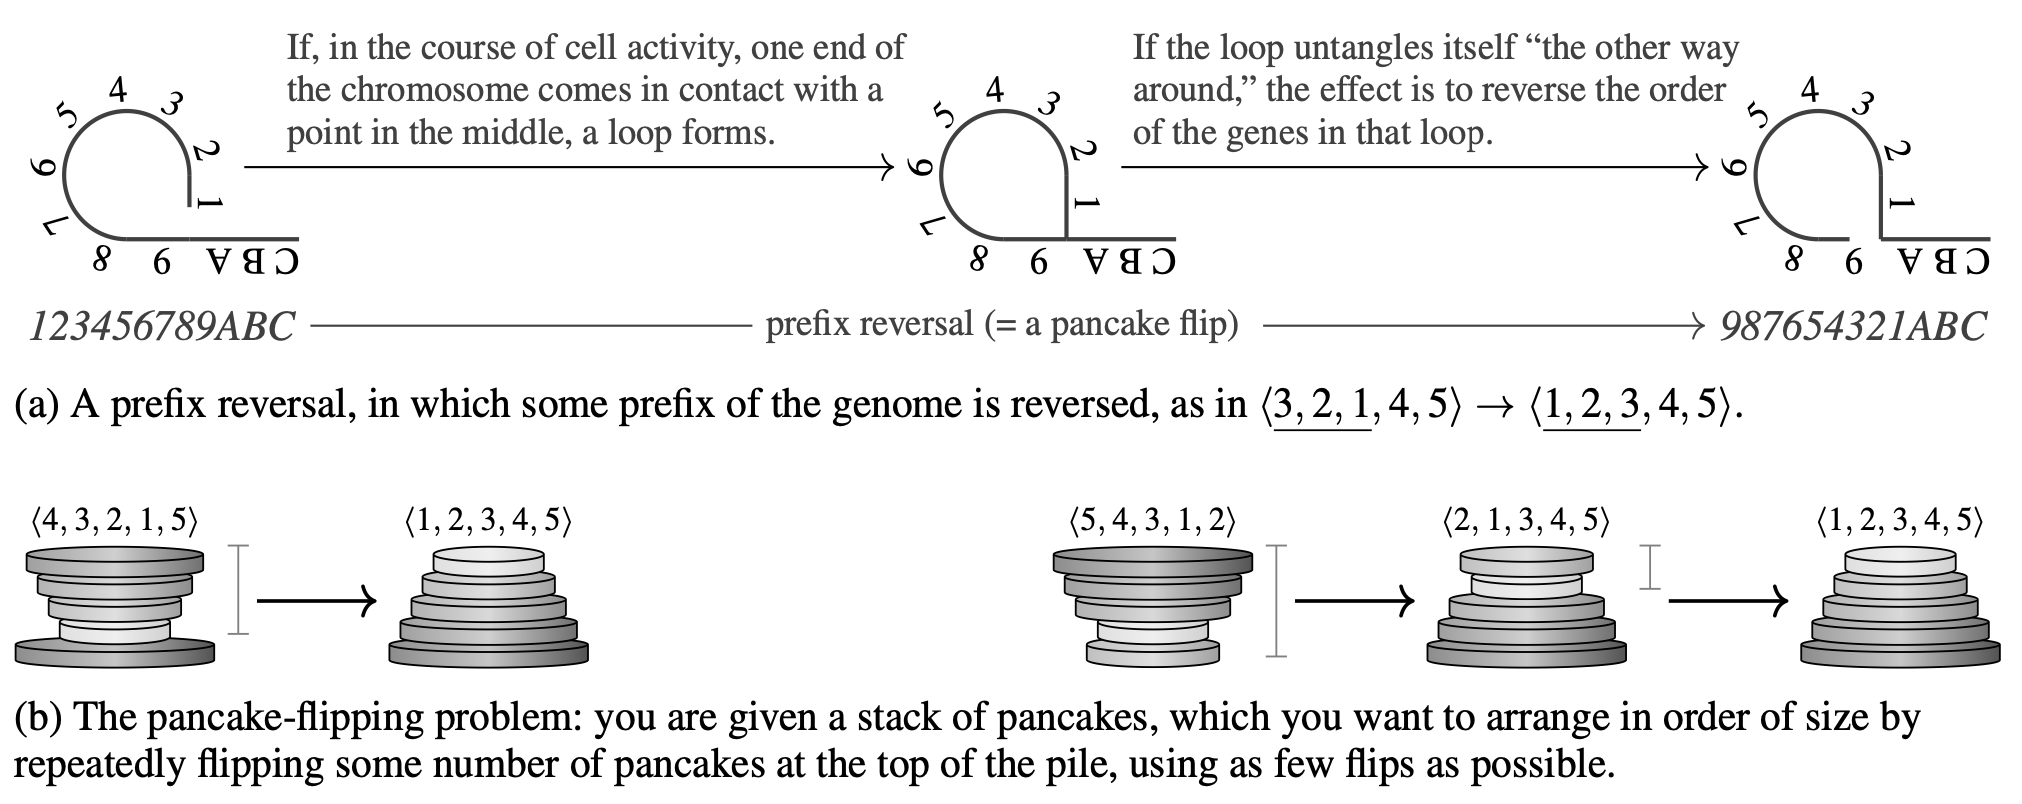
\includegraphics[width=\textwidth]{HW5_genome_pancake}
\caption{Genome rearrangements: prefix reversals and the pancake-flipping problem.}
\label{fig:HW5_bio_pancake}
\end{figure}

%3.189 & 190
\item Let $S$ be an arbitrary nonempty set and let $P$ be an arbitrary binary predicate. 
Decide whether the following statements are always true (for any $P$ and $S$), or whether they can be false. Prove your answers.
\begin{enumerate}
\item $[\exists y\in S: \forall x\in S:P(x,y)]\rightarrow [\forall x \in S: \exists y \in S:P(x,y)]$
\item $[\forall x \in S: \exists y \in S:P(x,y)]\rightarrow[\exists y \in S: \forall x \in S:P(x,y)]$
\end{enumerate}

\end{enumerate}
\end{document}